\documentclass[12pt]{article}
\usepackage{amsmath, amssymb, amsthm}
\usepackage{comment}
\usepackage{graphicx}
%\usepackage{savesym}
%\usepackage{color}
%\savesymbol{vec}
\usepackage{multirow}
\usepackage{array}
\usepackage{fullpage}
%\usepackage{natbib}
\usepackage{authblk}
\renewcommand\Authfont{\small}
\renewcommand\Affilfont{\itshape\small}
\normalfont
\usepackage[T1]{fontenc}
\usepackage{charter}
\renewcommand{\rmdefault}{ppl} % rm
\linespread{1.05}        % Palatino needs more leading
\usepackage[scaled]{helvet} % ss
\usepackage{courier} % tt
%%%%% macro for problem names and problem defn
\usepackage{xspace}
\newcommand{\ProblemFormat}[1]{{\sc #1}}
\newcommand{\ProblemIndex}[1]{\index{problem!\ProblemFormat{#1}}}
\newcommand{\ProblemName}[1]{\ProblemFormat{#1}\ProblemIndex{#1}\xspace}
\newcommand{\ProblemNameX}[2]{\ProblemFormat{#1}\ProblemIndex{#2}\xspace}
%\newcommand{\proboctlp}{\ProblemName{}}
%\usepackage[pdftex]{graphicx}
%\newtheorem{theorem}{Theorem}[subsection]
%\newtheorem{lemma}[theorem]{Lemma}
%\newtheorem{proposition}[theorem]{Proposition}
%\newtheorem{corollary}[theorem]{Corollary}
%\usepackage{mathtools}
\newtheorem{theorem}{Theorem}[subsection]
\newtheorem{lemma}[theorem]{Lemma}
\newtheorem{proposition}[theorem]{Proposition}
\newtheorem{corollary}[theorem]{Corollary}

%%%%%
\begin{document}
\title{Gesture Optimised Keyboard Layouts}
\author{Mohan Pednekar - CS15M064}
\affil[1]{Department of Computer Science and Engineering, Indian Institute of Technology Madras, India.\authorcr
\{mohanp\}@cse.iitm.ac.in}
\date{}
\maketitle
\begin{abstract}
Usage of standard 3 row Qwerty keyboard for touchscreens is a standard adopted from physical keyboards. Gesture based typing has emerged as a new way of typing on touchscreen. However standard Qwerty suffers from gesture ambiguity which is a problem non-relevant to touch typing. We are exploring some ways to design and test new as well as existing keyboard layouts to optimise them for touchscreen usage. The keyboards will be evaluated based on gesture speed and accuracy while minimising the ambiguity.

\end{abstract}
\newpage


\tableofcontents


\newpage

\section{Introduction}


Gesture typing is a very popular form of input in smartphones today. Keyboards like Swype, SwiftKey, SlideIT, TouchPal, and Google Keyboard are amongst the most popular ones which have gesture typing along with touch typing (tapping). Gestures let users develop muscle memory over time to create strokes for words they use most frequently. Usage of gestures eliminates the need to tap each letter. To accommodate words which cannot be recognised by the gestures, tapping is also available to facilitate traditional letter by letter input.




However, gesture typing suffers from ambiguous word gestures. The error rate for gesture typing is approximately 5-10\% \cite{evaluation} higher than for touch typing.  This problem occurs because when gesture typing, the input finger must inevitably cross unintended letters before reaching the intended one. The Qwerty layout amplifies this problem further because vowels such as u, i and o are arranged together on Qwerty, many pairs of words have
identical gestures, and many others have very similar gestures. An analysis of over a 40,000-word lexicon showed that 6.4\% of words have another word with an identical gesture on Qwerty.


The most straightforward solution would be to rearrange the keys on the keyboard to reduce duplicate or similar gestures. However, this will require users to learn the new layout first which may take time and defeat the whole purpose of optimising the layout.


We must also take into consideration the speed of making gesture. A lengthy gesture will require lot of time to complete the gesture. Even a gesture that is too short may force user to be precise and introduce speed reductions which appear counter-intuitive at first glance.


We will try to balance the above trade-offs while still reducing the gesture ambiguity in order to generate prototypes for gesture optimal keyboard layouts.


\section{Background Study}
\subsection{Dead zone based keyboards}
Cirrin \cite{cirrin} and Quikwriting \cite{quicwriting} were originally developed with a dead zone at the centre. They did not have the problem of gesture ambiguity since the user was expected to come back to the dead zone after each letter before going for the next letter. This had a huge drawback which is that the gestures were too long to be practical and often took more time than simple touch typing.

\subsection{Traditional row layout based keyboards}
Qwerty was originally developed to reduce jamming in typewriters by placing letters in most common bigrams far away from each other. But this problem is non-relevant to computer keyboards. Due to the popularity of Qwerty among all the existing typists, computer keyboards were also manufactured in Qwerty layout. Inherently, they were not optimised for comfortable typing. There were many alternative layouts created such as Dvorak, Colemak, Workman, Maltron, Typematrix etc. Some of them even have one handed layouts. Some gesture based keyboards also provide some of these as options for layout on touchscreen. However, it should be noted that although they are optimised for two handed typing using 8-10 fingers, they are not proven to be suitable for single finger gesture based typing. For example, Colemak is optimized mainly to retain AZXCV in their Qwerty positions to simplify clipboard operations. Dvorak is optimised to have all vowels on the left hand. These properties are undesirable in a gesture based keyboard. They exist primarily to help users use the same layout they use on their computers.


One of the most important problems with the usage of row layout based keyboards is that they create many gestures which have straight horizontal lines which results in many ambiguous and duplicate gestures. Hence the most effective solution would be to test the effect of slightly modified or staggered versions of existing keyboard layouts on the accuracy and speed of gesture typing and to use the results to incrementally test and revise better keyboard layouts until we achieve the target speed and accuracy.


\subsection{Existing Study on Gesture Optimised Keyboards}
Brian Smith, Xiaojun Bi, Shumin Zhai \cite{gesturerecog} have tried to tackle the problem and proposed 4 new keyboard layouts with different objectives as targets.

\begin{enumerate}

    \item GK-C: Clarity
    \item GK-S: Speed
    \item GK-D: Accuracy and Speed
    \item GK-T: Accuracy, Speed and Qwerty similarity
\end{enumerate}


\subsubsection{Procedure}
Since it is not possible to know how much weight needs to be given to each objective and also impossible to know what result to expect from the experiment, a dynamically adjustable technique need to be employed. A technique called Pareto optimisation had been successfully used in the past with good results. To do this, we find pareto optimal set (pareto front) of layouts in which none of its metric scores can be improved without hurting other scores. If there is a pareto superior layout, it replaces all the other layout it dominates. At each iteration, two randomly chosen keys are swapped. This is repeated sufficient number of times to calculate a sufficiently large pareto front. 

\begin{figure}[h!]
	\centering
	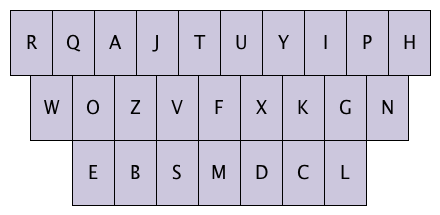
\includegraphics[scale=0.65]{Images/gkc}
	\caption{GK-C}
\end{figure}
\begin{figure}[h!]
	\centering
	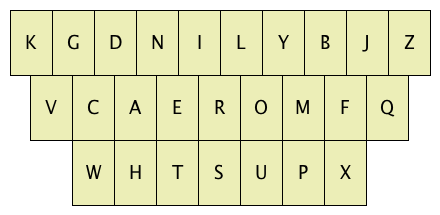
\includegraphics[scale=0.65]{Images/gks}
	\caption{GK-S}
\end{figure}
\begin{figure}[h!]
	\centering
	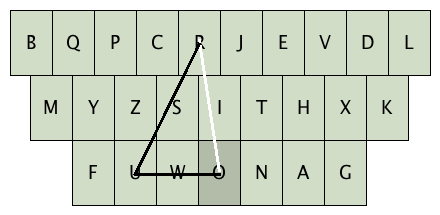
\includegraphics[scale=0.65]{Images/gkd}
	\caption{GK-D}
\end{figure}
\begin{figure}[h!]
	\centering
	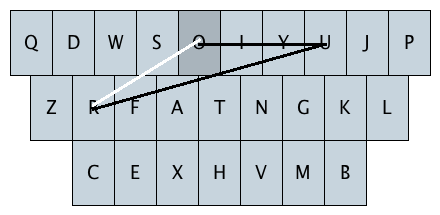
\includegraphics[scale=0.65]{Images/gkt}
	\caption{GK-T}
\end{figure}


\newpage
\subsubsection{Choosing the optimal layouts}
The pareto optimal set is usually represented using a multidimensional graph. However, for the purpose of the main problem to be solved, we can take the 2D cross section of the graph which is as follows. The layouts with best metric in a parameter are given the value 1.0 for that metric and other layouts are normalised with respect to that metric.


\begin{figure}[h!]
	\centering
	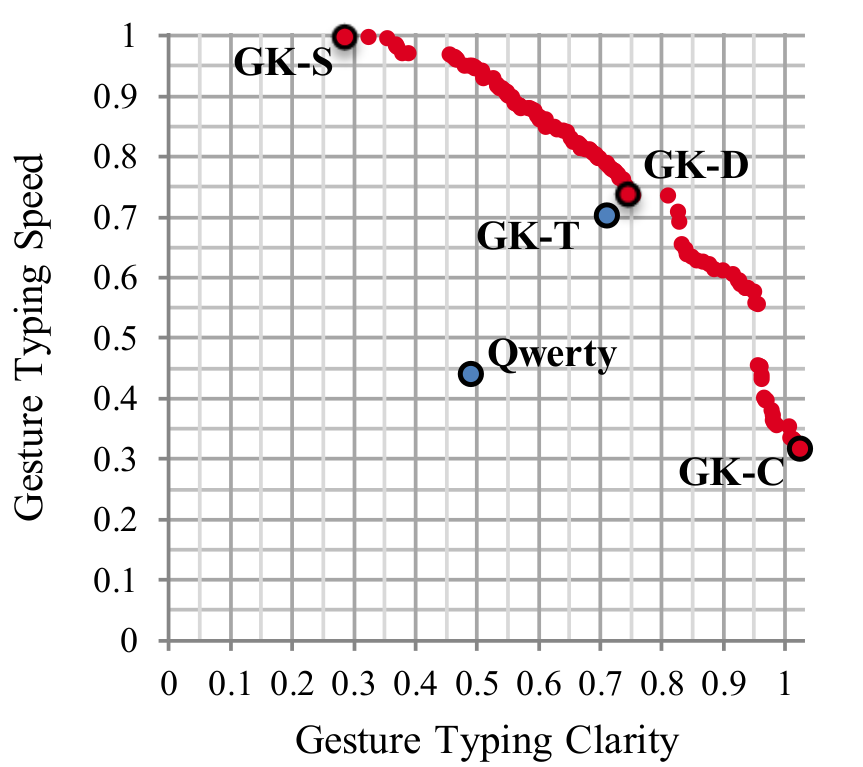
\includegraphics[scale=0.5]{Images/svc}
	\caption{2D Pareto Front}
\end{figure}


Once we get the normalised graph, the 45 degree point on the 2D graph is taken as double optimised layout GK-D.
The triple optimised layout GK-T is taken as a layout that lies closest to the 45 degree line on the 3D graph of pareto front.

\section{Metrics}
\subsection{Gesture Clarity}
We find the ideal trace for each word. This is a polyline connecting the midpoints of consecutive letters in the word. We find the nearest neighbour of each word. This is the word which will most likely conflict with the original word. We take average of the distance between each word and its nearest neighbour for all the words weighted by word frequency.

\[Clarity=\sum_{w \in L} f_{w} d_{w}\]
 \[ d_{w}= \min_{x \in L - \{w\} } d(w,x) \] 

 \[ \sum_{w \in L } f_{w} = 1\]

 \[ d(w,x) = \frac{1}{N} \sum_{i=1}^{N} \| w_{i} - x_{i} \|_{2} \]


\subsection{Gesture Speed}
Gestures are split into curves, line segments and corners. It was noticed that people tend to make faster strokes on longer line segments. The entry time for a stroke depends on the angle at a corner. However it was also noticed that this entry time was much smaller than the entry time for a line segment irrespective of curve. Hence it can be easily ignored. 
The total time required for the gesture can be simplified as the sum of times required by each segment and ignoring the small entry time of corners. 
Time required by each segment can be pre-calculated based on bigrams and the average time per bigram can be calculated for the entire layout using bigram frequency weights.

\[ T( \overline{AB} )= m \cdot (\| \overline{AB} \|_{2})^n   \]

\[ T(P)= \sum_{\overline{AB} \in P} T(\overline{AB}) \]

\[ o(i-j)= \sum_{w \in L} f_{w} \cdot (\text {\# occurunces of i-j in w}) \]

\[ G = \sum_{i,j \in \alpha} o(i-j) \cdot T(\overline{K_{i}K_{j}}) \]

\[ Speed = \frac{60000}{G} \]

\subsection{Qwerty Similarity}
The Qwerty similarity metric can be calculated using average of squared euclidean distances of keys from the the original Qwerty positions. However this metric is observed to punish farther placement of a small number of keys far more severely than a small displacement of multiple keys. Considering that keyboard is a grid, Manhattan distance was taken as a suitable metric to allow some infrequent keys to be moved more liberally without deeming the layout to be too dissimilar. To simplify Manhattan distance calculation, keys are aligned vertically by shifting middle row slightly to the left and bottom row to the right to align both of them to the top row.

\[ Similarity = \sum_{i \in \alpha} (|k_{i_{x}}-q_{i_{x}}| + |k_{i_{y}}-q_{i_{y}}|)\]


\section{Implementation}

\subsection{Metric Normalisation}
Tests are performed on each individual metric independently to estimate the maximum and minimum raw score for the metric.
10-30 optimisations are performed on each metric to achieve this.
Each optimisation starts with a random keyboard layout and runs for 2000 iterations swapping two random keys at each iteration.
Simulated annealing is used to keep better layouts with 100\% probability and other layouts with a fixed probability.
The normalised scores are used for the next phase.

\subsection{Pareto Front Initialisation}
22 different weightings are used for various linear combinations of metrics.
15 local neighbourhood searches are performed. Each search is 2000 iterations.
The objective is to maximise the score of the linear combinations.
The front is empty at first but each additional layout generated is added to the front as the pareto optimal layouts are found.


\subsection{Pareto Front Expansion}
200 passes are performed over the pareto front to find pareto optimal layouts similar to those in the pareto front.
Performing initialisation before this step helps in ensuring that all the possible solutions are reachable without swapping more than 2 keys at a time.

\subsection{Runtime}
For 40,000 words vocabulary, it took four machines with 32 threads each, three weeks to obtain the results.

\section{Modifications}
\subsection{Root level changes}
The existing layouts can be re designed with different number of rows or non linear arrangement of keys such as this layout called Interlaced Qwerty or iQwerty. This is a slight modification of original iQwerty proposal. The toggled middle row and quarter width extra alignment ensure that there are at most two characters in a straight diagonal trace. 
 
\begin{figure}[h!]
	\centering
	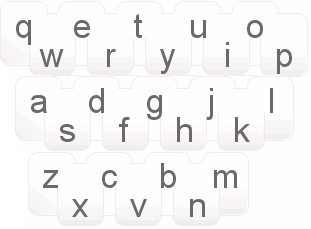
\includegraphics[scale=1]{Images/iqmod}
	\caption{Modified iQwerty}
\end{figure}
 
 
This layout reduces the number of linear duplicates significantly and contributes in both gesture clarity and speed. At the same time, it maintains Qwerty positions almost intact. Hence it can be used without incurring a significant learning curve.

\subsection{Metric changes}
\subsubsection{Gesture Clarity}
Calculating ideal trace as a series of straight line segments is not a realistic representative of human finger movements. Those can be better modelled using b-splines of appropriate order.
The proposed method is to generate a b-spline with n control points in the spline. One each at every character in the ideal trace. Each b-spline is split into 19 parts and pointwise distance from candidate trace at each split is recorded. Then we sum the distances of all 20 pairs and divide it by 20 to get the distance between the traces. We ignore all the words that start from a key farther than 1 unit away from the first letter of the candidate word and also those which end at a key farther than one unit away from the last letter. The word with the smallest distance from candidate word is the nearest neighbour. Inverse of the weighted average distance of all nearest neighbours is the the gesture clarity.

\subsubsection{Gesture Speed}
Usage of bigram-only model gives a representation of only line segments. We can use a combination of bigrams, trigrams and quad grams depending on the lengths of the words.
Such ngrams if more frequent will represent the muscle memory involved in making the stroke, effectively making those strokes faster than other strokes with similar score in bigram-only metric. Assuming that 'length' is the length of the trigram or quadgram, to calculate the time required, we use the formula $ time = 68.8 * length^{0.469} $. \cite{strokes}

\subsubsection{Qwerty Similarity}
There is a structural change in the layout. However, the we can still use finer grid to find Manhattan distance and divide the result by the number of grid cells per character. In this case, 4 grid cells. The euclidean divisor here would be $4 \sqrt{2}$. In order to compare any proposed layout with another. We need to divide the similarity by this euclidean divisor in order to maintain parity.

\subsection{Implementation changes}
Trigrams are used for words with lengths 4-7.
Quadgrams are used for all words longer than 6 letters.
These limits may be adjusted to represent frequency distribution accurately.

\section{Procedure}
\subsection{Corpus Processing}
Brown corpus is used as training data. It contains about 50,000 unique words.
Top 5000 most frequent words are used to generate n grams.
Ngram frequencies are calculated to find the most common n grams to be used for optimisation. For the purpose of testing, top 100 are used.

\subsection{Interface Quantisation}
Standard keyboard layout is used and key positions are calculated.
The centre of each key is considered as the key position.
The number of grid cells per key is multiplied by $\sqrt{2}$ to find the euclidean divisor of the layout.
Ideal trace is generated for all the words. 
This information is used to calculate nearest neighbour and also the gesture time length.
This process is repeated for structural change in the keyboard. Finer grid is used for modified iQwerty using 4 grid cells per key.

\subsubsection{B-Splines}
The traces are interpreted as b-Splines. To prune the dataset, the starting letter of the at the first control point is considered as unchanged and all the other traces are ignored. This is likely to be true because generally users choose the first character more precisely than rest of the characters in the stroke. Gesture entry time is expected to be directly proportional to Qwerty similarity. However, this hypothesis has not been tested since we are testing the metrics per layout basis instead of testing the layout optimality.

\section{Observations}
Distance between two b-splines is currently calculated using control points. Ideally we would need about 20 points to calculate distances with close to 90\% accuracy. To be able to propose new keyboard layout, we should consider 40 points in order to make more accurate predictions (close to 96\%) in approximately double the amount of time.
 
\begin{figure}[h!]
	\centering
	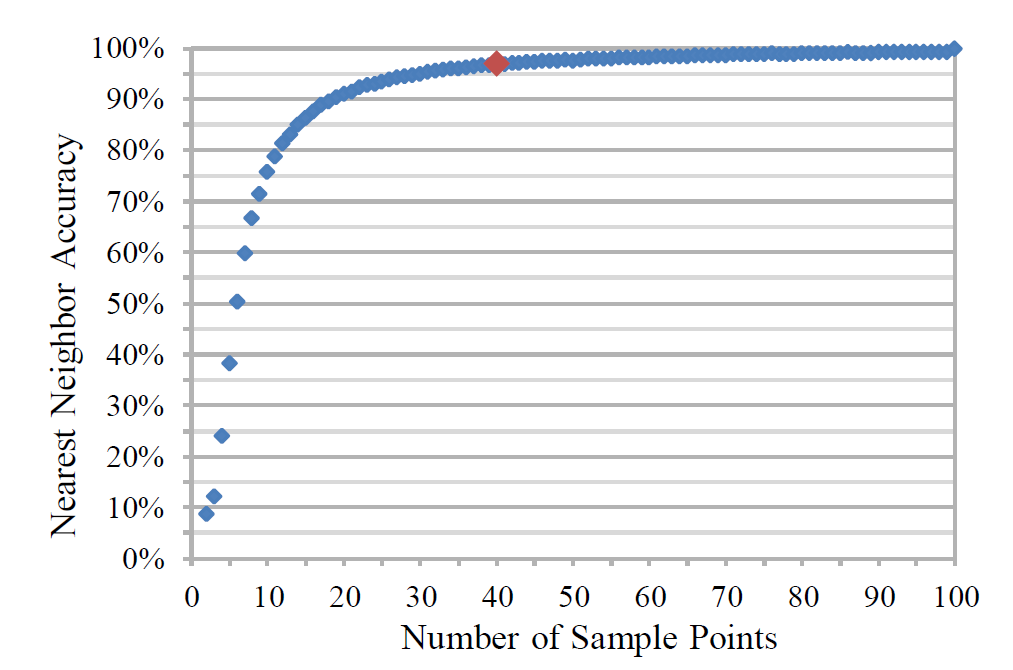
\includegraphics[scale=0.5]{Images/accuracy}
	\caption{Accuracy v/s Sample points }
\end{figure}

 However, to prove the superiority of improved metrics over the older metrics, we performed distance calculations for randomly chosen 100 words at a time with their own ideal traces. 100 words each were chosen from 4 to 10 letter words. Here, ideal trace is the b-spline of the order n-1. Older metric is straight lines connecting consecutive letters. New metric is replacing common trigrams or quadgrams with b-splines.

 
\begin{figure}[h!]
	\centering
	\includegraphics[scale=1]{Images/prob}
	\caption{Probability of getting closer to ideal trace}
\end{figure}
 
 

The new metric shows distance closer to zero than the old metric for all the tested word lengths with greater than 90\% probability. 7 being 100\% for trigrams, 9 and 10 being 100\% each for quadgrams.

\section{Conclusion}
The results achieved so far can be used to propose new keyboard layouts and can have further refinements in stroke sampling and processing. The results shall also be tested on users to check whether they follow the experimental assumptions about speed, accuracy and familiarity. Pareto front calculation and expansion using new metrics will give more realistic results since the measured difference between ideal and improved metrics is smaller than that with old metrics.


\begin{thebibliography}{10}
\bibitem{gesturerecog} 
Brian A. Smith1 Xiaojun Bi Shumin Zhai,
\textit{Optimizing Touchscreen Keyboards for Gesture Typing}. 
CHI 2015.
 
\bibitem{cirrin} 
Mankoff, J. and Abowd, G.D.  
\textit{Cirrin: a word-level unistroke keyboard for pen input.}
In Proc. UIST 1998, ACM Press (1998), 213 - 214.
 
\bibitem{quicwriting} 
Perlin, K. 
\textit{Quikwriting: continuous stylus-based text entry.} 
In Proc. UIST 1998, ACM Press (1998), 215 - 216.

\bibitem{evaluation}
Bi, X., Azenkot, S., Partridge, K., and Zhai, S. 
\textit{Octopus: evaluating touchscreen keyboard correction and recognition algorithms via remulation}
In Proc. CHI 2013, ACM Press (2013), 543 - 552

\bibitem{strokes}
Cao, X. and Zhai, S. 
\textit{Modeling human performance of pen stroke gestures.}
In Proc. CHI 2007, ACM Press (2007), 1495–1504.

\end{thebibliography}

\end{document}
